%!TEX root = presentation.tex
\usetheme{Berlin}
\usecolortheme{beaver}

\usepackage[utf8]{inputenc}
\usepackage[T1]{fontenc}
\usepackage{lmodern}

\usepackage{listings}
\usepackage{graphicx}
\usepackage{float}
\usepackage{caption}
\captionsetup{labelformat=empty,labelsep=none}

\usepackage{color}
\newcommand{\hilight}[1]{\colorbox{yellow}{#1}}

\usepackage[backend=bibtex, 
firstinits=true,
style=numeric]{biblatex}
\addbibresource{bibliography.bib}

\setbeamertemplate{bibliography item}{%
  \ifboolexpr{ test {\ifentrytype{book}} or test {\ifentrytype{mvbook}}
    or test {\ifentrytype{collection}} or test {\ifentrytype{mvcollection}}
    or test {\ifentrytype{reference}} or test {\ifentrytype{mvreference}} }
    {\setbeamertemplate{bibliography item}[book]}
    {\ifentrytype{online}
       {\setbeamertemplate{bibliography item}[online]}
       {\setbeamertemplate{bibliography item}[article]}}%
  \usebeamertemplate{bibliography item}}

\defbibenvironment{bibliography}
  {\list{}
     {\settowidth{\labelwidth}{\usebeamertemplate{bibliography item}}%
      \setlength{\leftmargin}{\labelwidth}%
      \setlength{\labelsep}{\biblabelsep}%
      \addtolength{\leftmargin}{\labelsep}%
      \setlength{\itemsep}{\bibitemsep}%
      \setlength{\parsep}{\bibparsep}}}
  {\endlist}
  {\item}


\title{Presentation\\
Gilbert: A sparse linear algebra environment}
\author[T. Rohrmann]{Till Rohrmann\\
\texttt{till.rohrmann@campus.tu-berlin.de}}
\institute[TUB]{Technische Universität Berlin}
\date{\today}
\subject{Gilbert: A sparse linear algebra environment}

\begin{document}
		\frame{\titlepage}
		\begin{frame}
			\frametitle{Table of Contents}
			\tableofcontents
		\end{frame}
		\section{Motivation}

\begin{frame}
	\frametitle{Demand for big data analytics}
	\begin{itemize}
		\item More and more data gathered
		\item Companies want to exploit the gathered data to obtain new insights
		\begin{itemize}
			\item Crime site prediction
			\item Recommender systems
		\end{itemize}
		\item Data grows exponentially
		\item Analytic methods have to scale up as well
	\end{itemize}
\end{frame}

\begin{frame}
	\frametitle{Ways to scale up}
	\begin{enumerate}
		\item Develop new algorithm
		\item Increase computer performance
		\item Run in parallel
	\end{enumerate}
\end{frame}

\begin{frame}
	\frametitle{Data analytic methods}
	\begin{itemize}
		\item Many data analytic and machine learning algorithms based on linear algebra
		\item Developed with linear algebra systems, such as Matlab, R, Octacve, etc.
		\begin{itemize}
			\item + Easy to code and test -> Quick development
			\item + Huge existing code base
			\item - Explicit parallelization
		\end{itemize}
	\end{itemize}
\end{frame}

\begin{frame}
	\frametitle{Distributed computing systems}
	\begin{itemize}
		\item Explicit parallelization, such as OpenMP and MPI, tedious and error-prone
		\item New parallel programming paradigms emerged, MapReduce, Spark, Stratosphere, Pregel, etc.
		\item Frees from low-level parallelization tasks
		\item Requires to adhere to a certain programming model
	\end{itemize}
\end{frame}

\begin{frame}
	\frametitle{Distributed computing systems and data analytics}
	\begin{itemize}
		\item Intersection of people familiar with both domains is really small
		\item Laborious to become acquainted with new domain
		\item Tedious to transform existing algorithms to new programming model
		\item Can't we bring both worlds together?
		\item Solution: Gilbert
	\end{itemize}
\end{frame}
		\section{Gilbert}

\begin{frame}
	\frametitle{Gilbert}
	\begin{itemize}
		\item Sparse linear algebra system
		\item Matlab frontend for distributed computing frameworks
		\item Allows to almost seamlessly move from local execution to distributed execution in a heterogenous environment
		\item Enable machine learning and data analytics algorithm to be run on web-scale data 
	\end{itemize}
\end{frame}
		\section{Approach}

\begin{frame}
	\frametitle{Approach}
	\begin{columns}
		\begin{column}{0.6\textwidth}
			\begin{enumerate}
				\item Compiling Matlab code into intermediate representation
				\item Apply optimizations indenpendently of runtime specific system
				\item Compiling intermediate representation into runtime specific format
			\end{enumerate}
		\end{column}
		\begin{column}{0.4\textwidth}
			\includegraphics[width=0.8\textwidth]{images/approach.jpg}
		\end{column}
	\end{columns}
\end{frame}

\begin{frame}
	\frametitle{System architecture}
	\begin{center}
		\includegraphics[height=0.8\textheight]{images/architecture.png}
	\end{center}
\end{frame}

\begin{frame}[fragile]
	\frametitle{Language}
	\begin{columns}
		\begin{column}{0.65\textwidth}
			\begin{itemize}
				\item Matlab-like language
				\item Support of basic linear algebra operations
				\item Some built-in functions, repmat, linspace, pdist2
				\item Loop support with static and dynamic termination criterion
				\item Language expressive enough to support variety of algorithms, Pagerank, K-means, NNMF
			\end{itemize}
		\end{column}
		\begin{column}{0.35\textwidth}
			\begin{lstlisting}[basicstyle=\scriptsize]
A'*B

f=@(x) x.^2.0

eps = 0.1

c=@(p,c) norm(p-c,2) < eps

fixpoint(1/2, f, 10, c)
			\end{lstlisting}
		\end{column}
	\end{columns}
\end{frame}

\begin{frame}
	\frametitle{Compilation: Intermediate format}
	\begin{itemize}
		\item Scala's combinator parsing tool box
		\item Powerful enough for our language
		\item Matlab is dynamically typed
		\item Execution on Stratosphere requires type knowledge at compilation time
		\item Hindley-Milner type inference algorithm to infer types and dimensions
	\end{itemize}
\end{frame}

\begin{frame}[fragile]
	\frametitle{Example: Parsing and typing}
	\begin{block}{Input}
\begin{lstlisting}[language=Matlab]
A = ones(2,10);
B = eye(10,3);
A*B
\end{lstlisting}
\end{block}
	
\begin{block}{Parsed and typed}	
\begin{lstlisting}[language=Matlab]
A = ones(2,10):MatrixType[Double,2,10];
B = eye(10,3):MatrixType[Double,10,3];
A*B:MatrixType[Double,2,3]
\end{lstlisting}
\end{block}

\end{frame}

\begin{frame}[fragile]
	\frametitle{Example: Intermediate code}
	\begin{block}{Compiled}
\begin{lstlisting}[columns=flexible, language=Java]
MatrixMult(
  ones(
    IntValue(2),
    IntValue(10)
  ), 
  eye(
    IntValue(10),
    IntValue(3)
  )
)
\end{lstlisting}
	\end{block}
\end{frame}

\begin{frame}
	\frametitle{Example: Stratosphere execution plan}
	\begin{center}
		\includegraphics[height=0.9\textheight]{images/matrixMultDataflow.png}
	\end{center}
\end{frame}
		\section{Current state}

\begin{frame}
	\frametitle{Current state}
	\begin{itemize}
		\item Language layer working (except for the typing algorithm which is still a little bit buggy)
		\item Execution on Stratosphere with iteration and convergence support
		\item PageRank, NNMF and K-means executable
	\end{itemize}
\end{frame}

\begin{frame}
	Live demonstration
\end{frame}		
		%!TEX root = presentation.tex
\section{Outlook}

\begin{frame}
	\frametitle{Outlook}
	\begin{columns}
		\begin{column}{0.6\textwidth}
			\begin{itemize}
				\item Typing system with constraints, similar to Haskell typing system with type class support
				\item System evaluation: Runtime, scalability
				\item Comparison to specialized algorithms
				\item Optimizations for the intermediate representation
			\end{itemize}
		\end{column}
		\begin{column}{0.4\textwidth}
			\includegraphics[width=\textwidth]{images/outlook.jpg}
		\end{column}
	\end{columns}
\end{frame}
		%!TEX root = presentation.tex
\section{Related Work}

\begin{frame}
\frametitle{Related Work}
	\begin{columns}
		\begin{column}{0.7\textwidth}
			\begin{itemize}
				\item SystemML~\cite{ghoting:2011a}
				\begin{itemize}
					\item Higher-level language for linear algebra
					\item Compiled to MapReduce jobs 
				\end{itemize}
				\item Apache Mahout~\cite{apache:a2011}
				\begin{itemize}
					\item Specialized implementations of algorithms of various kind
					\item No native linear algebra support
				\end{itemize}
				\item Pegasus~\cite{kang:2009a}
				\begin{itemize}
					\item Generalized iterative matrix vector multiplication
				\end{itemize}
				\item Spark~\cite{zaharia:2010a}
				\begin{itemize}
					\item MapReduce extension
				\end{itemize}
			\end{itemize}
		\end{column}
		\begin{column}{0.3\textwidth}
			\includegraphics[width=\textwidth]{images/bookPile.jpg}
		\end{column}
	\end{columns}

\end{frame}	
		\begin{frame}[allowframebreaks]
  \frametitle<presentation>{Bibliography}
  \nocite{*}
  \bibliographystyle{amsalpha}
  \bibliography{bibliography}
\end{frame}

		%!TEX root=presentation.tex
\section*{}

\begin{frame}
	\frametitle{Replication based matrix multiplication}
	\begin{center}
	\includegraphics[width=\textwidth]{images/rmm.png}
	\end{center}
\end{frame}	

\begin{frame}
	\frametitle{Cross product based matrix multiplication}
	\begin{center}
	\includegraphics[height=0.8\textheight]{images/cpmm.png}
	\end{center}
\end{frame}

\begin{frame}
	\frametitle{Communication costs}
	\begin{itemize}
		\item Matrix $A$ blocked with $M \times K$ blocks and $B$ blocked with $K \times N$ blocks
		\item Network and IO costs are dominant
		\item $costs_{RMM} \in O\left(network(|A|\cdot N + |B|\cdot M) + io(|A|+|B|+|C|)\right)$
		\item $costs_{CPMM} \in O\left(network(|A|+|B|+r\cdot|C|) + io(|A|+|B|+|C|) \right)$ with $r$ being the number of reducer
	\end{itemize}
\end{frame}

\begin{frame}
	\frametitle{Stratosphere execution plan}
	\begin{columns}
		\begin{column}{0.5\textwidth}
			\begin{itemize}
				\item Assuming row-wise partitioning of matrix $A$
				\item Execution plans for RMM and CPMM identical
				\item Differ only in chosen strategy for join operator
				\item RMM: Hybrid-hash join
				\item CPMM: Sort-merge join
				\item Stratosphere's optimizer chooses right plan
			\end{itemize}
		\end{column}
		\begin{column}{0.5\textwidth}
			\includegraphics[width=0.9\textwidth]{images/matrixMult.png}
		\end{column}
	\end{columns}
\end{frame}
\end{document}
